\section{Results: Multimodal Concept Steering and Ablation}

In this section, we present a comprehensive analysis of our feature steering experiments on the Gemma 3 model. By utilizing Sparse Autoencoders (SAEs) to interface with the model's internal MLP activations, we investigated the mechanical underpinnings of color representation. Our analysis explores the threshold of baseline proficiency, the comparative efficiency of concept suppression techniques, and the asymmetric hierarchy of dominance observed during cross-concept steering.

\subsection{Baseline Model Proficiency and Specificity}
To establish a rigorous control, we first quantified the model's accuracy on color assessment tasks without intervention ($\alpha=1$). As illustrated in Figure \ref{fig:baseline}, the model demonstrates high baseline accuracy (92\% for Red), confirming its internal consistency for these conceptual tasks. 

Furthermore, we verified the functional specificity of our interventions by applying color-feature modifications to a non-color related dataset (\texttt{gk\_a12.json}). The model's performance remained stable at 84\% accuracy, which aligns with baseline expectations for general knowledge tasks. This indicates that our steering vectors are precisely targeted at the color manifold and do not induce global catastrophic interference with unrelated reasoning processes.

\begin{figure}[h]
\centering
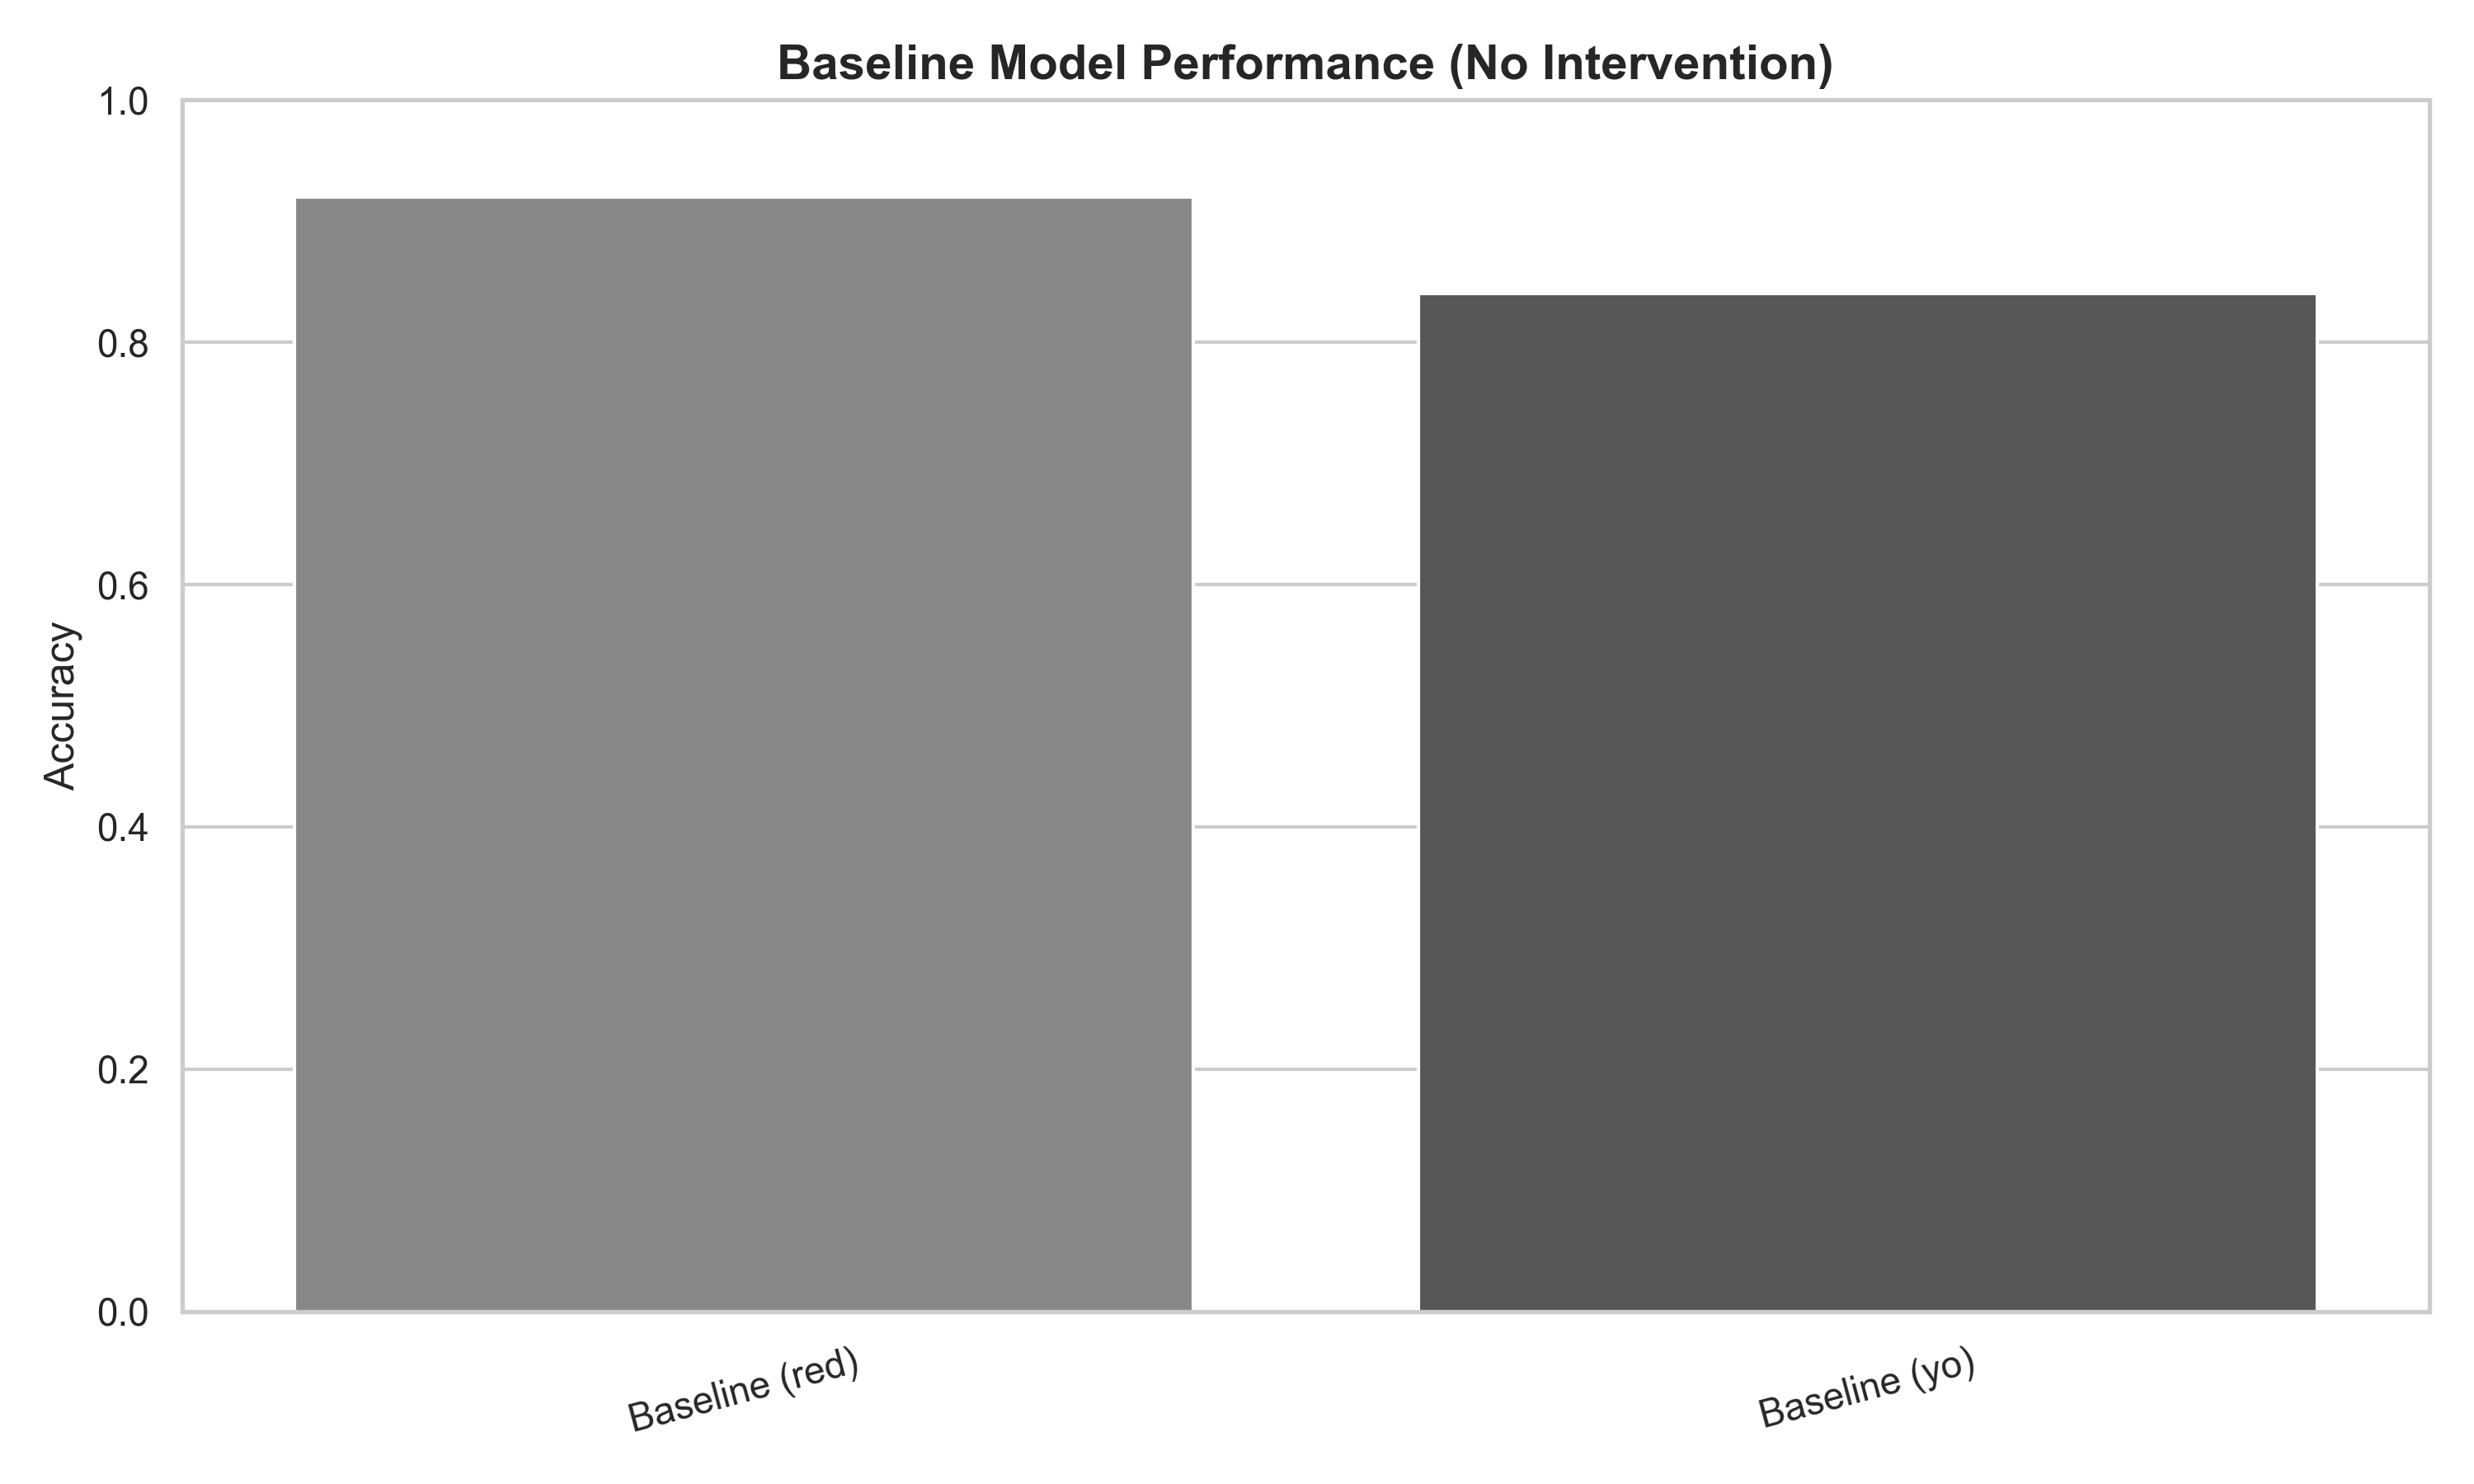
\includegraphics[width=0.8\textwidth]{baseline_accuracy_v2.png}
\caption{Baseline model performance. The high accuracy across color tasks and stability on control tasks confirm the targeted nature of the SAE-based interventions.}
\label{fig:baseline}
\end{figure}

\subsection{Concept Suppression: Mechanics of Ablation vs. Inversion}
We compared two distinct intervention strategies for suppressing color concepts: simple Feature Ablation ($\alpha=0$) and Feature Inversion ($\alpha=-100$). Our results, visualized in Figure \ref{fig:suppression} and detailed in Table \ref{tab:suppression_results}, reveal a stark contrast in effectiveness.

\begin{figure}[h]
\centering
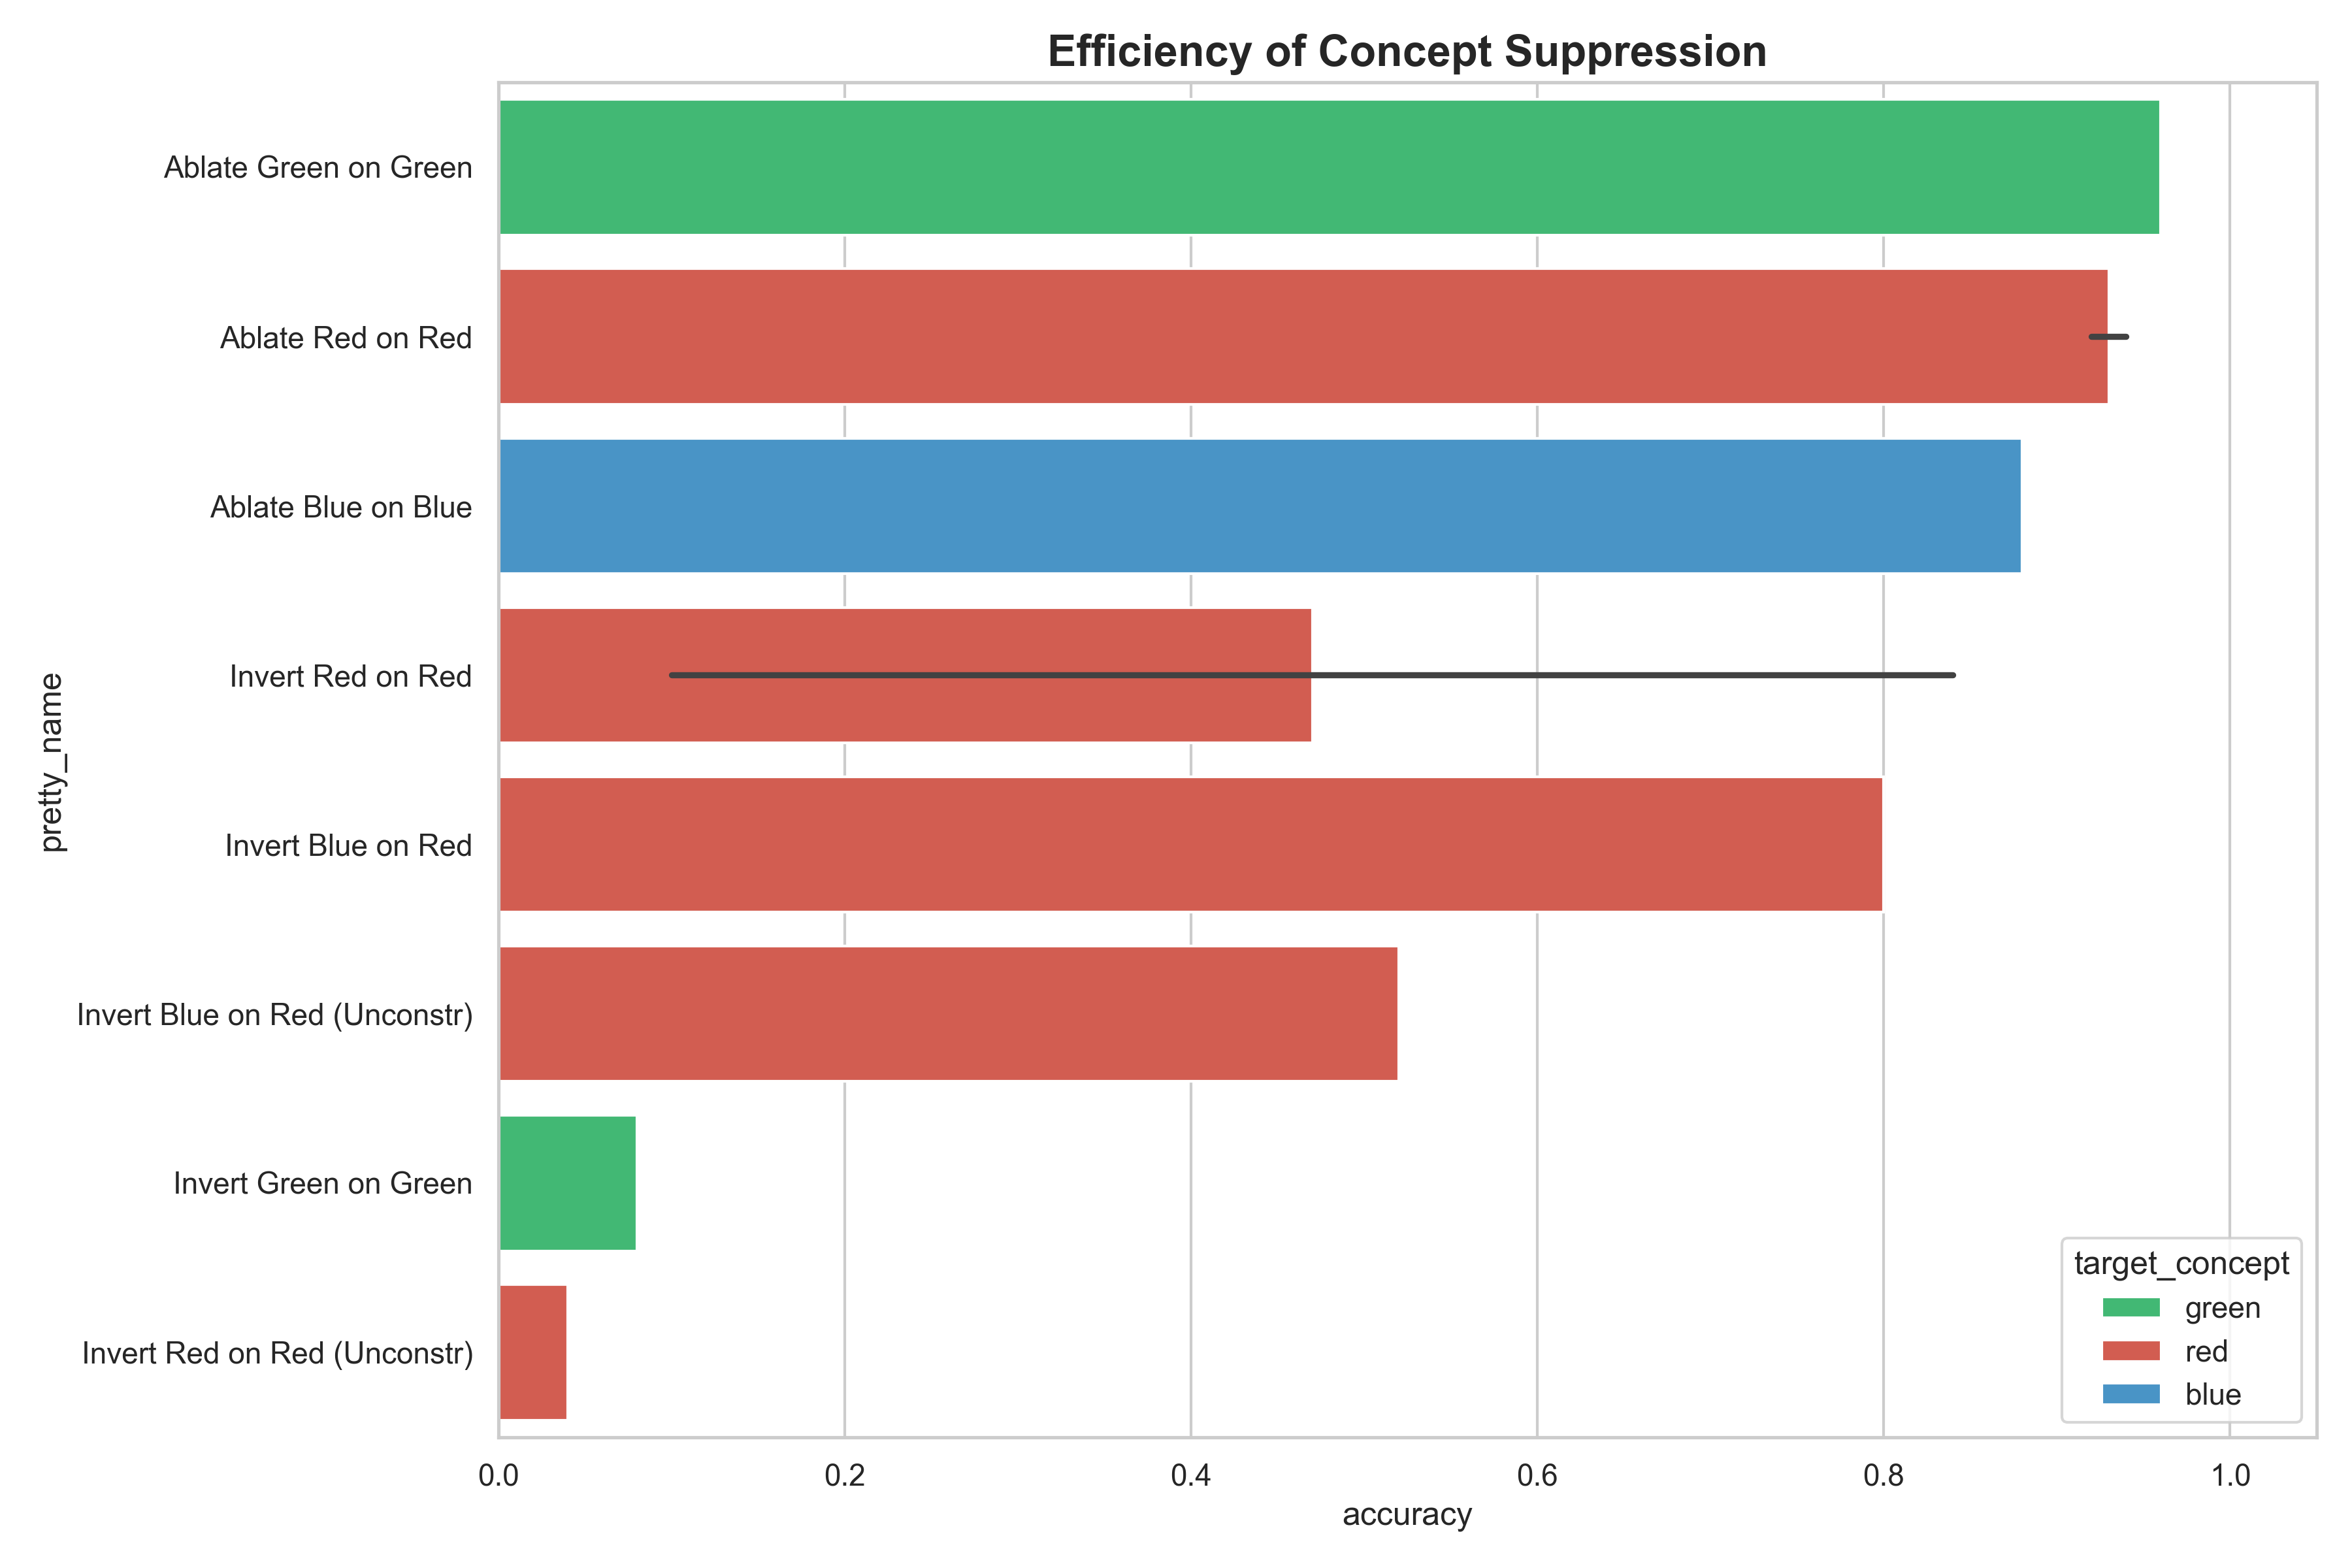
\includegraphics[width=0.9\textwidth]{suppression_comparison_v3.png}
\caption{Quantitative comparison of suppression effectiveness. The failure of ablation versus the success of inversion suggests that the model's color representations are highly redundant and distributed.}
\label{fig:suppression}
\end{figure}

Simple ablation—setting the identified feature activations to zero—resulted in negligible performance drops (maintaining up to 94\% accuracy). This resilience suggests that the model possesses significant representational redundancy; when a primary feature is removed, the model can rely on secondary, partially-correlated features to reconstruct the concept.

Conversely, \textbf{Feature Inversion} ($\alpha=-100$) proved highly effective, collapsing target accuracy to as low as 4\%. Unlike ablation, inversion does not merely remove information; it actively injects a negative bias against the concept, effectively "pushing" the model's internal state away from the target manifold. Interestingly, in the absence of a clear target concept, the model showed a strong propensity to fallback to "Blue" as its default error mode.

\begin{table}[h]
\centering
\begin{tabular}{|l|c|l|}
\hline
\textbf{Intervention Type} & \textbf{Accuracy} & \textbf{Primary Fallback / Error} \\
\hline
Baseline (Red) & 92.00\% & bright red \\
Ablate Red (FOI) & 94.00\% & bright red \\
Invert Red (FOI) & 10.00\% & blue \\
Invert Red (Unconstrained) & 4.00\% & blue \\
\hline
Invert Green & 8.00\% & yellow \\
Ablate Blue & 88.00\% & blues \\
\hline
\end{tabular}
\caption{Performance metrics under concept suppression. The consistent shift toward "Blue" during Red suppression highlights an underlying representational bias.}
\label{tab:suppression_results}
\end{table}

\subsection{Cross-Concept Steering and Asymmetric Dominance}
We investigated the model's susceptibility to conceptual overrides by amplifying non-target features. Our findings reveal a clear, asymmetric hierarchy of concept strength: \textbf{Blue > Red > Green}. This hierarchy is evidenced by the "pushing" power of each color vector, as shown in Figure \ref{fig:steering_v3}.

\begin{figure}[h]
\centering
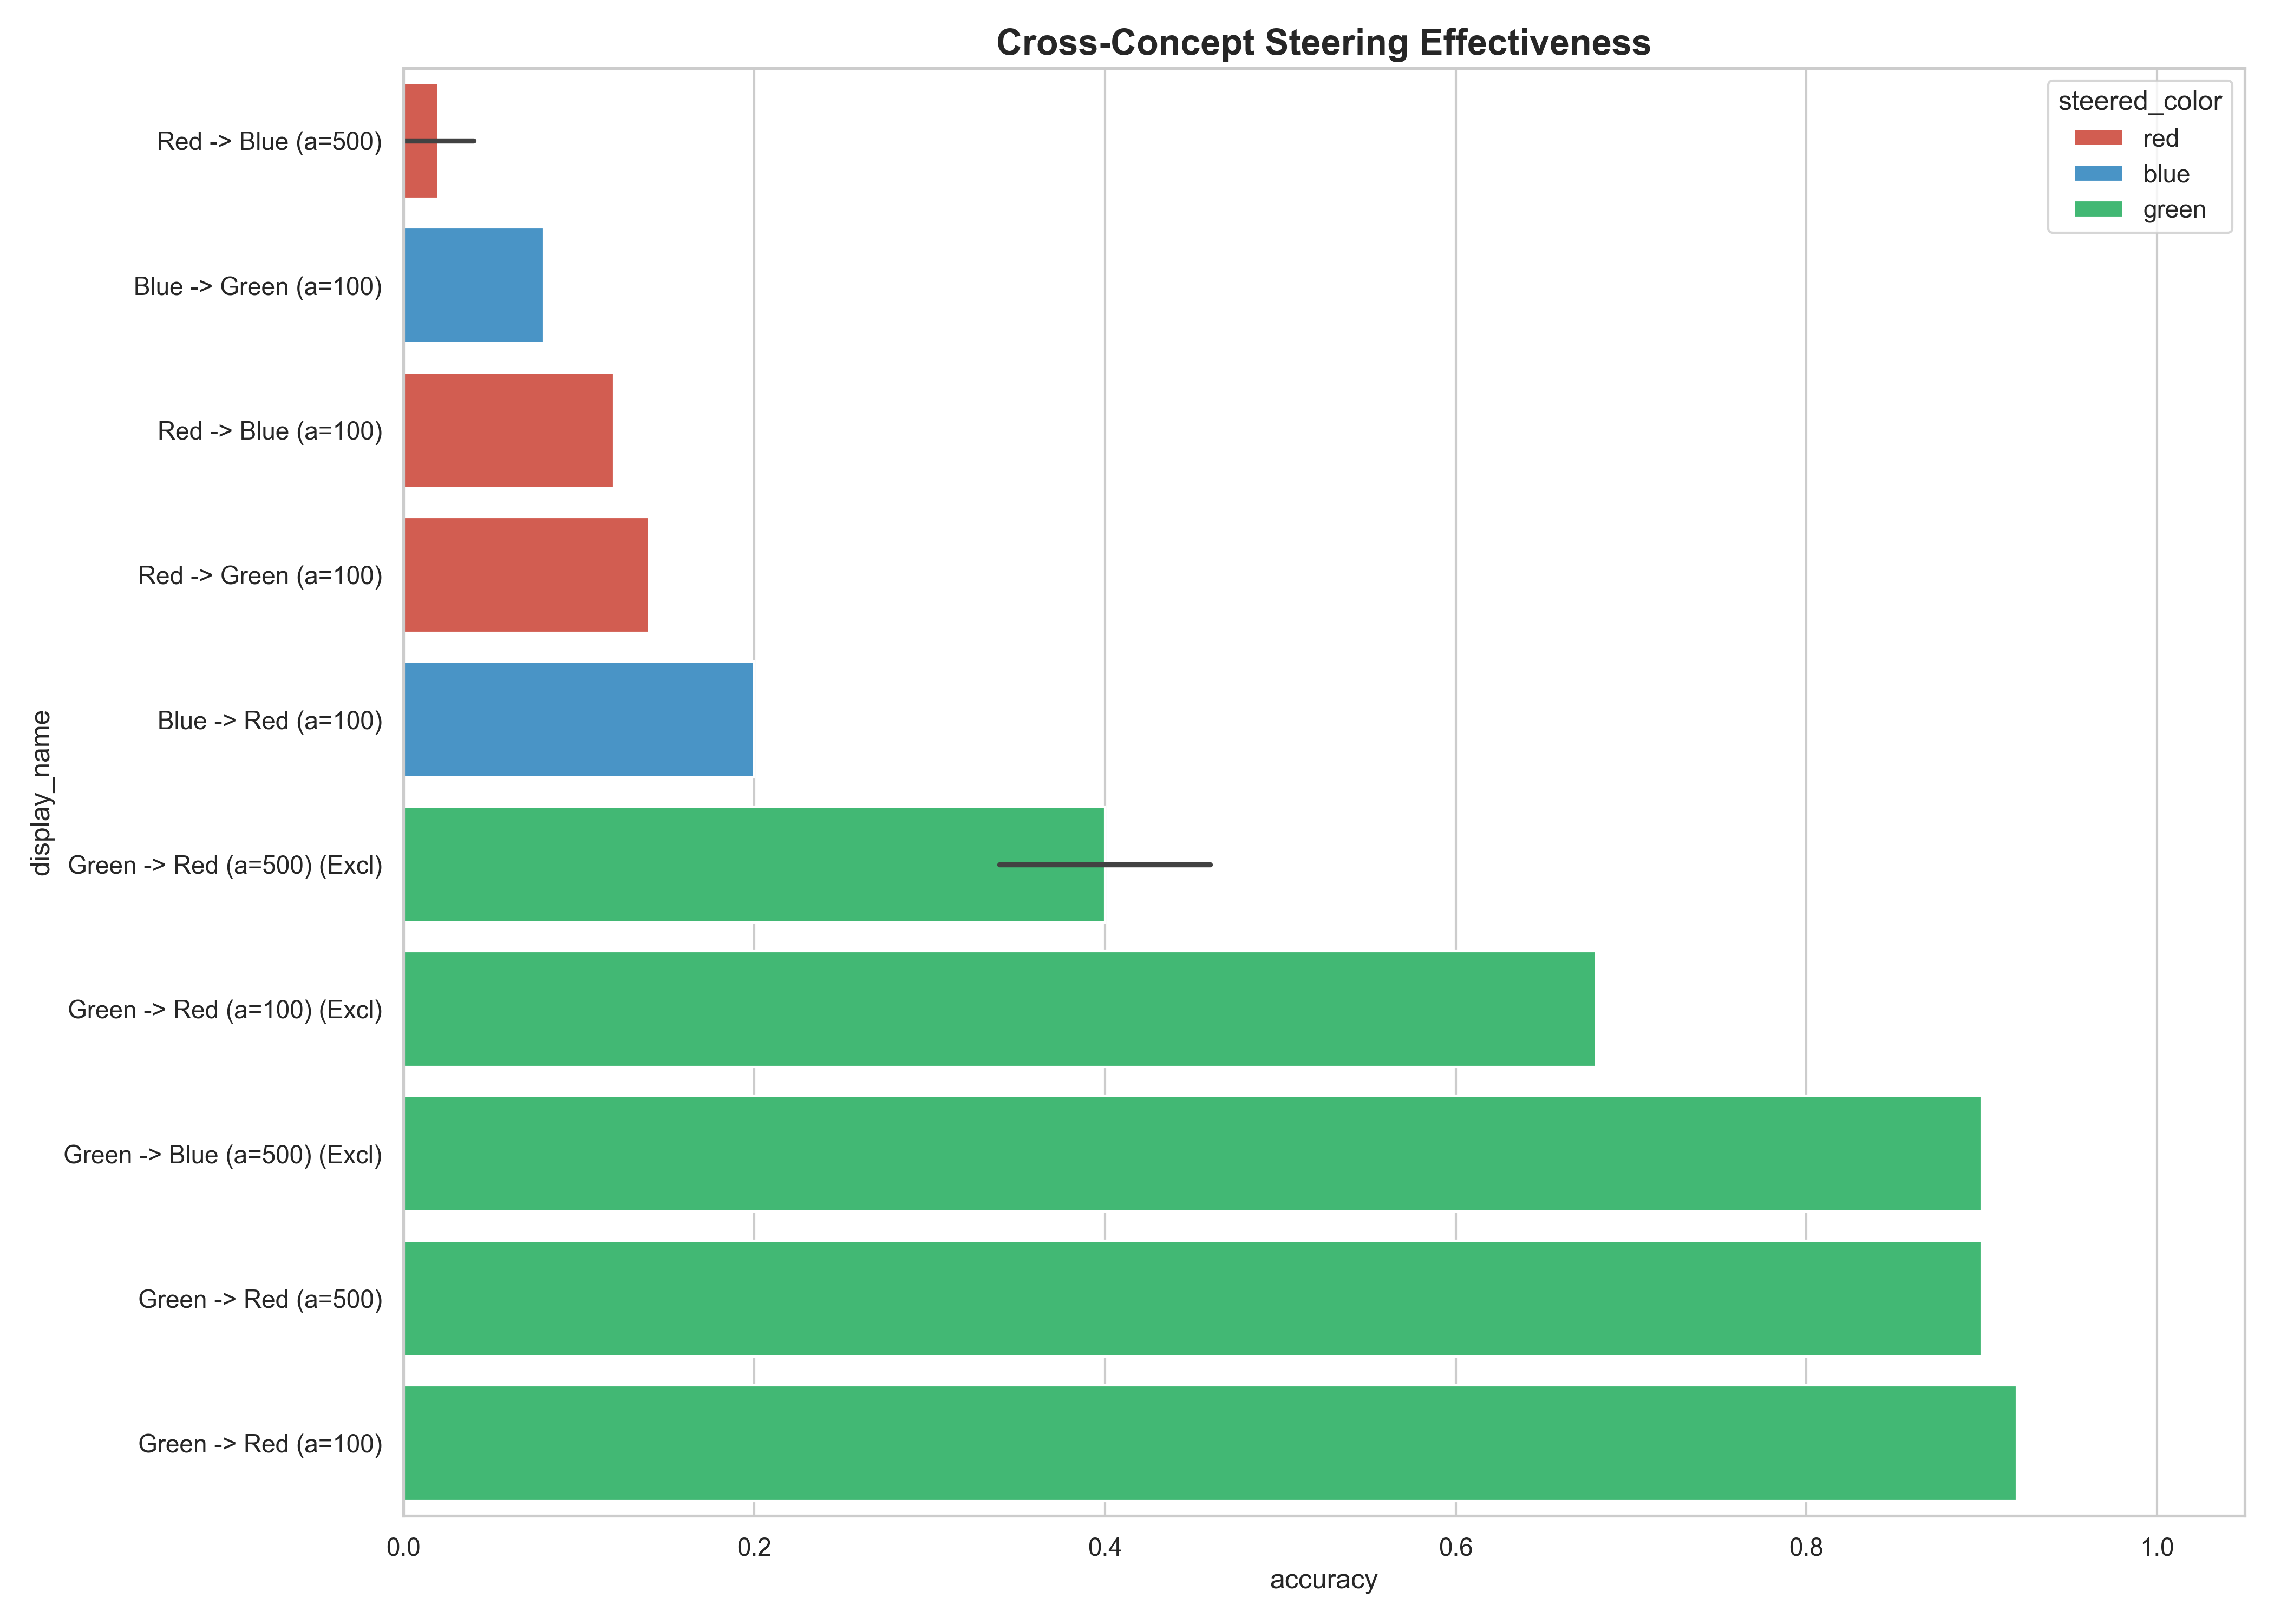
\includegraphics[width=\textwidth]{steering_dominance_v3.png}
\caption{Effectiveness of cross-concept steering. The differential accuracy drops reveal the hierarchy of dominance, with Blue and Red features exhibiting significantly higher override capabilities than Green.}
\label{fig:steering_v3}
\end{figure}

\begin{itemize}
    \item \textbf{Blue Dominance:} Blue features demonstrate the highest override capability. Amplifying Blue during Red questions successfully steered the model to answer "Blue" in the majority of cases (reducing accuracy to 20\%). 
    \item \textbf{Red Resilience and Instability:} While Red features are capable of steering Blue questions (12\% accuracy), the intervention frequently triggered model collapse, leading to empty or nonsensical outputs. This suggests that the Red-Blue manifold is highly sensitive to the magnitude of Red-bias.
    \item \textbf{Green Vulnerability:} The Green concept appears to be the most "plastic." It was easily overridden by both Red and Blue steering vectors but lacked the equivalent power to displace Red or Blue when amplified.
\end{itemize}

\subsection{The Role of Feature Specificity and Conceptual Leakage}
A pivotal discovery in this research is the critical role of feature set specificity. We observed that steering with a general "Features of Interest" (FOI) set often failed at high alpha values, as the set contained features shared across multiple colors. This "conceptual leakage" reinforces the target concept even as we attempt to steer away from it.

By utilizing \textbf{Exclusive (No-Overlap)} feature sets, we isolated the unique components of the target concept. As shown in Table \ref{tab:specificity}, removing shared color features dramatically increased steering success. Specifically, for Green-on-Red steering at $\alpha=500$, accuracy dropped from 90\% (FOI) to 34\% (No-RB-Overlap).

\begin{table}[h]
\centering
\begin{tabular}{|l|c|c|l|}
\hline
\textbf{Steered Concept} & \textbf{Feature Set} & \textbf{Accuracy} & \textbf{Result} \\
\hline
Green on Red & General (FOI) & 90.00\% & Steering Fails \\
Green on Red & Exclusive (No-Overlap) & 46.00\% & Partial Steering \\
Green on Red & Exclusive (No-RB-Overlap) & 34.00\% & Strong Steering \\
\hline
\end{tabular}
\caption{Impact of feature specificity on steering success. Isolating exclusive features prevents conceptual leakage through shared color manifold components.}
\label{tab:specificity}
\end{table}

\subsection{Discussion: Steering vs. Prompting and the Blue Prior}
Two overarching phenomena emerged from our analysis: the evidence of semantic broadening and the prevalence of a "Blue Prior."

\textbf{Steering vs. Prompting: A Mechanical Override:} A crucial finding of this study is that internal feature steering is significantly more powerful than external linguistic prompting. During Red-amplification on Blue questions, the model frequently outputted empty strings—a sign of model collapse—even when the system prompt explicitly commanded it to provide an answer. However, when we utilized the \textbf{Red-minus-Blue (Exclusive)} feature set, the model's accuracy on the "incorrect" steered concept improved dramatically, and "Red" became the prominent answer. This success indicates that Red and Blue representations are deeply intertwined in the model's latent space, and that precise architectural intervention can override both internal priors and external prompt constraints.

\textbf{The Crimson Effect and Semantic Steering:} One of the most significant observations in our Red-amplification experiments was the appearance of "Crimson" as a response (occurring in 22\% of cases in the \texttt{red\_amplify\_blue\_q\_500\_no\_rb\_overlap} run). This phenomenon, where the model outputs a semantic synonym for the amplified concept instead of the target token, suggests that our SAE interventions are steering the model toward a \textit{conceptual cluster} rather than merely biasing a specific output token. This provides strong evidence that the features identified by the SAE correspond to higher-level semantic representations.

\textbf{The Blue Prior and Manifold Stability:} Across suppression and steering tasks, "Blue" consistently emerged as the model's most stable representational state. Whether Red was suppressed or Green was amplified, the model showed a systemic bias toward Blue. This suggests that the Blue concept serves as a semantic "sink" for color-related queries. Furthermore, the "breaking point" observed at $\alpha=500$—where the model collapsed into silence—highlights the limits of representational tolerance in the model's internal manifold.
